\documentclass[tikz]{standalone}
\usetikzlibrary{shapes.geometric, arrows, positioning, backgrounds}

\tikzstyle{object} = [
text centered,
draw=black,
fill=lightgray,
text=black,
rectangle,
minimum width=3cm, 
minimum height=1cm,
align=center]

\tikzstyle{connector} = [
draw=black,
thick]

\tikzstyle{semiconnector} = [
draw=black,
line width=3pt,
dotted,
thick]

\tikzstyle{arrow} = [
draw=black,
thick,
->]

\tikzstyle{semiarrow} = [
draw=black,
line width=3pt,
dotted,
thick,
->]

\begin{document}
  
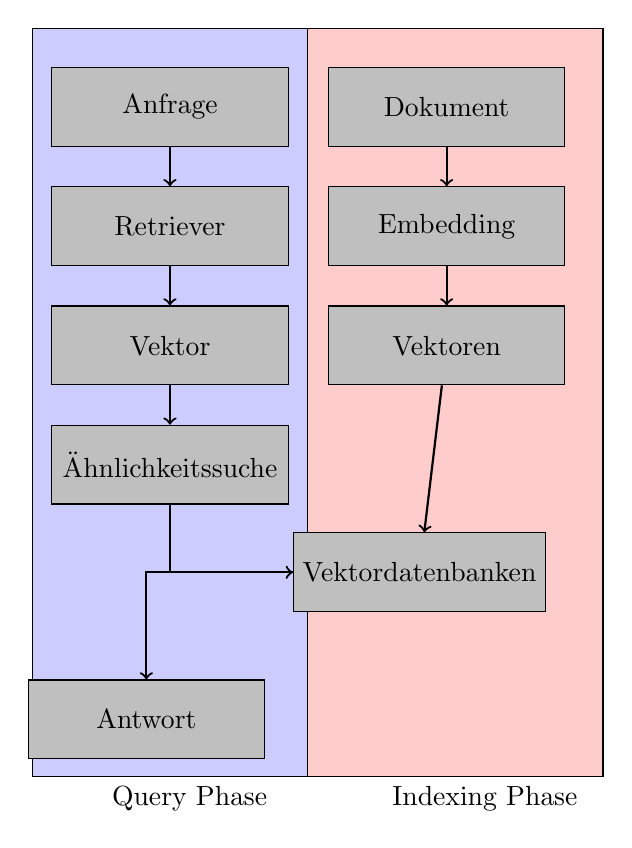
\begin{tikzpicture}[node distance=0.5cm]

\node[object] (query) {Anfrage};
\node[object, below =of query] (embeddingQuery) {Retriever};
\node[object, below =of embeddingQuery] (queryVektor) {Vektor};
\node[object, below =of queryVektor] (similaritySearch) {Ähnlichkeitssuche};
\node[object, right =of query] (document) {Dokument};
\node[object, right =of embeddingQuery] (embeddingDoc) {Embedding};
\node[object, right =of queryVektor] (dataVectors) {Vektoren};
\node[object, below right =of similaritySearch, xshift=-0.3cm] (database) {Vektordatenbanken};
\node[object, below left =of database, yshift=-0.5cm] (result) {Antwort};

\draw[arrow] (query) -- (embeddingQuery);
\draw[arrow] (embeddingQuery) -- (queryVektor);
\draw[arrow] (queryVektor) -- (similaritySearch);
\draw[arrow] (similaritySearch) |- (database);
\draw[arrow] (document) -- (embeddingDoc);
\draw[arrow] (embeddingDoc) -- (dataVectors);
\draw[arrow] (dataVectors) -- (database);
\draw[arrow] (database) -| (result);

\begin{scope}[on background layer]
\draw[fill=blue!20] (-1.75,1) rectangle (1.75,-8.5)
    node[below, xshift=-1.5cm] {Query Phase};

\draw[fill=red!20] (1.75,1) rectangle (5.5,-8.5)
    node[below, xshift=-1.5cm] {Indexing Phase};
\end{scope}

\end{tikzpicture}
\end{document}